\documentclass[14pt, a4paper]{extarticle}
\usepackage{GOST}
\usepackage{array}
\usepackage{verbatim}
\usepackage[detect-all]{siunitx}
\usepackage{amsmath}
\usepackage{amssymb}
\usepackage[utf8]{inputenc}
\usepackage{hyperref}
\usepackage{tempora}

\makeatletter
\renewcommand\@biblabel[1]{#1.}
\makeatother

\usepackage{listings}
\lstset{ 
	language=python,
	basicstyle=\small\sffamily, 
	numbers=left, 
	numberstyle=\tiny,
	stepnumber=1,
	numbersep=5pt,
	showspaces=false,            
	showstringspaces=false,      
	showtabs=false,             
	frame=single,            % рисовать рамку вокруг кода
	tabsize=4,      
	commentstyle=\color{green},
	keywordstyle=\color{blue}\textbf,
	numberstyle=\scriptsize\color{gray}, % the style that is used for the line-numbers
	rulecolor=\color{black},
	captionpos=t,
	breaklines=true,         % автоматически переносить строки 
	breakatwhitespace=false, % переносить строки по пробелу
	escapeinside={\#*}{*)} 
}

\begin{document}
	
\begin{table}[ht]
	\centering
	\begin{tabular}{|c|p{400pt}|} 
		\hline
		\begin{tabular}[c]{@{}c@{}} 
\includegraphics[scale=1]{baum.jpg} \\\end{tabular} &
		\footnotesize\begin{tabular}[c]{@{}c@{}}\textbf{Министерство~науки~и~высшего~образования~Российской~Федерации}\\\textbf{Федеральное~государственное~бюджетное~образовательное~учреждение}\\\textbf{~высшего~образования}\\\textbf{«Московский~государственный~технический~университет}\\\textbf{имени~Н.Э.~Баумана}\\\textbf{(национальный~исследовательский~университет)»}\\\textbf{(МГТУ~им.~Н.Э.~Баумана)}\\\end{tabular}  \\
		\hline
	\end{tabular}
\end{table}
\noindent\rule{\textwidth}{4pt}
\noindent\rule[14pt]{\textwidth}{1pt}
\hfill 
\noindent
\makebox{ФАКУЛЬТЕТ~}%
\makebox[\textwidth][l]{\underline{~«Информатика и системы управления»~~~~~~~~~~~~~~~~~~~~~~~~~~~~~~~~~}}%
\\
\noindent
\makebox{КАФЕДРА~}%
\makebox[\textwidth][l]{\underline{~«Операционные системы»~}}%


\begin{center}
	\vspace{1.5cm}
	{\bf\huge Отчёт\par}
	{\bf\Large по лабораторной работе № 5\par}
	\vspace{0.7cm}
\end{center}

\noindent
\makebox{\large{\bf Название:}~~~}
\makebox[\textwidth][l]{\large\underline{~ Буферизованный и не буферизованный ввод-вывод~}}\\


\noindent
\makebox{\large{\bf Дисциплина:}~~~}
\makebox[\textwidth][l]{\large\underline{~Операционные системы~}}\\

\vspace{1.5cm}
\noindent
\begin{tabular}{l c c c c c}
	Студент      & ~ИУ7-65Б~               & \hspace{2.5cm} & \hspace{2cm}                 & &  Д.В. Сусликов \\\cline{2-2}\cline{4-4} \cline{6-6} 
	\hspace{3cm} & {\footnotesize(Группа)} &                & {\footnotesize(Подпись, дата)} & & {\footnotesize(И.О. Фамилия)}
\end{tabular}

\noindent
\begin{tabular}{l c c c c}
	Преподователь & \hspace{5cm}   & \hspace{2cm}                 & & ~~~Н.Ю. Рязанова~~~\\\cline{3-3} \cline{5-5} 
	\hspace{3cm}  &                & {\footnotesize(Подпись, дата)} & & {\footnotesize(И.О. Фамилия)}
\end{tabular}

\vspace{0.6cm}
\begin{center}	
	\vfill
	\large \textit {Москва, 2021}
\end{center}

\thispagestyle {empty}
\pagebreak

% ВВЕДЕНИЕ
\clearpage
\textbf{Программа 1} \par




%\begin{figure}[h]
%	\centering
%	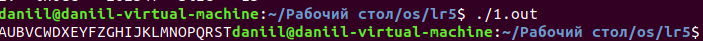
\includegraphics[scale=1]{graphics/1.png}\\ Зависимость температуры от координаты в разные моменты времени при l = %10, x от 0 до 10.
%\end{figure}\par
%\


\textbf{Листинг:}
\begin{lstlisting}
def k(T):
	return a1 * (b1 + c1 * T ** m1)

def c(T):
	return a2 + b2 * T ** m2 - c2 / T ** 2

def alpha(x):
	d = (alphaN * l) / (alphaN - alpha0)
	c = - alpha0 * d
	return c / (x - d)

def p(x):
	return 2 / R * alpha(x)

def f(x):
	return 2 * T0 / R * alpha(x)

def func_plus_1_2(x, step, func):
	return (func(x) + func(x + step)) / 2

def func_minus_1_2(x, step, func):
	return (func(x) + func(x - step)) / 2

def A(T):
	return (k(T) + k(T - tau)) * tau / h / 2

def D(T):
	return (k(T) + k(T - tau)) * tau / h / 2

def B(x, T):
	return A(T) + D(T) + c(T) * h + p(x) * h * tau

def F(x, T):
	return f(x) * h * tau + c(T) * T * h

def run_through(prevT):
	(c(prevT[0]) + c(prevT[0] + tau)) / 2

	K0 = h / 8 * (c(prevT[0]) + c(prevT[0] + tau)) / 2 + h / 4 * c(prevT[0]) + \
	(k(prevT[0]) + k(prevT[0] + tau)) / 2 * tau / h + \
	tau * h / 8 * p(h / 2) + tau * h / 4 * p(0)
	
	M0 = h / 8 *  (c(prevT[0]) + c(prevT[0] + tau)) / 2 - \
	(k(prevT[0]) + k(prevT[0] + tau)) / 2 * tau / h + \
	tau * h * p(h / 2) / 8
	
	P0 = h / 8 * (c(prevT[0]) + c(prevT[0] + tau)) / 2 * (prevT[0] + prevT[1]) + \
	h / 4 * c(prevT[0]) * prevT[0] + \
	F0 * tau + tau * h / 8 * (3 * f(0) + f(h))
	
	KN = h / 8 * (c(prevT[-1]) + c(prevT[-1] - tau)) / 2 + h / 4 * c(prevT[-1]) + \
	(k(prevT[-1]) + k(prevT[-1] - tau)) / 2 * tau / h + tau * alphaN + \
	tau * h / 8 * p(l - h / 2) + tau * h / 4 * p(l)
	
	MN = h / 8 * (c(prevT[-1]) + c(prevT[-1] - tau)) / 2 - \
	(k(prevT[-1]) + k(prevT[-1] - tau)) / 2 * tau / h + \
	tau * h * p(l - h / 2) / 8
	
	PN = h / 8 * (c(prevT[-1]) + c(prevT[-1] - tau)) / 2 * (prevT[-1] + prevT[-2]) + \
	h / 4 * c(prevT[-1]) * prevT[-1] + tau * alphaN * T0 + \
	tau * h / 4 * (f(l) + f(l - h / 2))


	eps = [0, -M0 / K0]
	eta = [0, P0 / K0]
	
	x = h
	n = 1
	while (x + h < l):
	eps.append(D(prevT[n]) / (B(x, prevT[n]) - A(prevT[n]) * eps[n]))
	eta.append((F(x, prevT[n]) + A(prevT[n]) * eta[n]) / (B(x, prevT[n]) \
	- A(prevT[n]) * eps[n]))
	n += 1
	x += h
	
	y = [0] * (n + 1)
	y[n] = (PN - MN * eta[n]) / (KN + MN * eps[n])
	
	for i in range(n - 1, -1, -1):
	y[i] = eps[i + 1] * y[i + 1] + eta[i + 1]
	
	return y

def iter_method():
	result = []
	n = int(l / h)
	T = [T0] * (n + 1)
	newT = [0] * (n + 1)
	ti = 0
	
	result.append(T)
	
	while (True):
		buf = T
		while True:
			newT = run_through(buf)
			if check_iter(buf, newT):
				break
			buf = newT
		
		result.append(newT)
		ti += tau
		if (not check_eps(T, newT)):
			break
		
		T = newT
	
	return result, ti

def check_eps(T, newT):
	for i in range(len(T)):
		if fabs((T[i] - newT[i]) / newT[i]) > 1e-2:
			return True
	return False

def check_iter(T, newT):
	max = fabs((T[0] - newT[0]) / newT[0])
	for i in range(len(T)):
		d = fabs(T[i] - newT[i]) / newT[i]
		if d > max:
			max = d
	return max < 1

\end{lstlisting}

\end{document}









